\documentclass[runningheads]{llncs}
\usepackage[T1]{fontenc}
\usepackage{graphicx}
\usepackage{booktabs}
\newcommand{\corr}{(*)}
% N.B.: do not change anything above this line. If you require additional packages, please load them directly after this line.
% \usepackage{mwe} % optional

% Add extra packages here (after the line above)
\usepackage{amsmath,amssymb} 
\usepackage{cleveref}
\usepackage{algorithm}
\usepackage{algpseudocode} 
\usepackage{tikz}
\usepackage{url}
 
\IfFileExists{xcolor.sty}{\usepackage{xcolor}}{\usepackage{color}}
\definecolor{dpgCritical}{rgb}{1.000,0.851,0.400}      % #ffd966
\definecolor{dpgPredBranch}{rgb}{0.714,0.843,0.659}    % #b6d7a8
\definecolor{dpgCompBranch}{rgb}{0.957,0.800,0.800}    % #f4cccc
\definecolor{dpgFocus}{rgb}{0.624,0.773,0.910}         % #9fc5e8
\definecolor{dpgContext}{rgb}{0.973,0.976,0.984}       % #f8f9fb
\definecolor{dpgTrueLeaf}{rgb}{0.576,0.769,0.490}      % #93c47d
\definecolor{dpgOtherLeaf}{rgb}{0.902,0.722,0.686}

\usetikzlibrary{positioning,arrows.meta} 


\begin{document}

\title{Decision Predicate Graphs for Local Diagnostic Analysis of Tree-Ensemble Decisions Beyond Output Agreement}

\titlerunning{DPGs for Local Diagnostic Analysis}

% For double-blind submission (recommended for initial review), use:
% \author{Author information scrubbed for double-blind reviewing}
% \authorrunning{Anonymous Authors}

% Camera-ready version (uncomment when not double-blind)
\author{Author information scrubbed for double-blind reviewing}
\authorrunning{Anonymous Authors}
\institute{}

\maketitle
\begin{abstract} %max 2000 chars
Output-level agreement is an insufficient criterion for local explanations when the goal is to diagnose how a model reached a specific decision, since two explanations can match a prediction equally well while differing substantially in path-level faithfulness. We address this through Decision Predicate Graphs (DPGs), extending the original global construction to DPG-local, which builds each explanation as a sample-specific subgraph from the exact root-to-leaf paths executed by the ensemble. On top of this structure, a Semantic Graph View provides diagnostic quantities including explanation confidence, support margin, competitor exposure, vote agreement, and conditional critical-node descriptors. Across 15 benchmark datasets, near-complete trace recovery (edge recall $\approx$ 0.99) confirms structural faithfulness, while edge precision and zero recombination serve as construction-consistency checks. The diagnostics identify disagreement and difficult regimes: low confidence predicts local disagreement with AUROC about $0.90$, vote agreement is even stronger, and many-class or high-dimensional datasets such as \texttt{isolet}, \texttt{digits}, and \texttt{madelon} expose clear limits. DPG-local is therefore positioned as a structure-aware diagnostic layer for tree-ensemble decisions, complementary to output-aligned explainers such as TreeSHAP, LIME, Anchors, LORE-style local surrogates, and path baselines.
\keywords{Explainable AI \and Local explanations \and Tree ensembles \and Random forests \and Decision Predicate Graphs \and Structural faithfulness}
\end{abstract}

\section{Introduction}
Explainable AI methods are commonly distinguished by the scope of the explanation they provide. Global explanations aim to characterise the behaviour of the predictive model as a whole, whereas local explanations are designed to explain a single prediction or the model's behaviour in the neighbourhood of a specific instance \cite{lundberg2020local,vilone2021notions,setzu2021glocalx}. Local explanations are especially important in decision-support settings because inspection, validation, contestability, and error analysis often arise at the level of an individual case rather than only at the level of aggregate model behaviour \cite{nauta2023anecdotal}.
Many widely used local explanation methods are optimised for \emph{prediction-level} faithfulness and express explanations primarily through \emph{input features} or feature conditions. Local Interpretable Model-agnostic Explanations (LIME), for instance, explain a prediction by fitting an interpretable surrogate in the neighbourhood of the query point, whereas Shapley Additive exPlanations (SHAP) decompose the prediction into additive feature contributions relative to a reference baseline \cite{ribeiro2016why,lundberg2017unified}. Related methods, such as Individual Conditional Expectation (ICE) and Anchors, likewise describe local behaviour through feature-wise sensitivity profiles or sufficient rule conditions \cite{goldstein2015ice,ribeiro2018anchors}. Since ICE is a response-profile diagnostic rather than a route or path explainer, we report it separately in Appendix~\ref{app:ice} instead of using it as a main structural baseline. In Fr\"amling's terminology, these methods predominantly characterise \emph{feature influence}, that is, effects defined with respect to a baseline or perturbation distribution, rather than the broader notion of feature importance \cite{framling2023importanceinfluence}.
This perspective is useful, but insufficient for the problem targeted in this research. When the objective is to inspect how a model arrived at a specific inference, diagnose failure modes, or compare competing class hypotheses, fidelity, understood as the degree to which an explanation accurately reflects its behaviour \cite{vilone2021notions}, is too weak a criterion when only assessed at the final output level. Different local explanations may exhibit similar prediction-level fidelity but differ substantially in preserving the executed decision path and exposing the diagnostically relevant local decision structure.

\begin{figure}
    \centering
    \includegraphics[width=1\linewidth]{high-level-diagram.png}
    \caption{High-level diagram of the Decision Predicate Graphs complemented by the Semantic Graph View for structured local explanations}
    \label{fig:high-level-d}
\end{figure}

In this research article, we investigate the hypothesis that \emph{Decision Predicate Graphs} (DPG) can serve as a faithful and informative basis for local explanations of tree-ensemble predictions, because they encode a model inferential process directly at the level of standardised split predicates and their empirically observed transitions \cite{arrighi2024decision}. 
Accordingly, we represent each local explanation as a sample-specific graph obtained from the predicates activated by the ensemble for the inspected instance. In this representation, nodes correspond to \emph{predicates} extracted from tree internal splits, that is, interpretable feature-value tests of the form $(x_j \leq \theta)$ (or $(x_j > \theta)$), where thresholds are mapped to a common vocabulary through rounding and consistent predicate formatting. 
Edges represent \emph{predicate transitions} activated along executed root-to-leaf paths, capturing the local ordering and co-occurrence of split conditions that lead to the predicted outcome.
Our central thesis is that local graph explanations should be evaluated not only by agreement with the model output, but also by how well they recover the executed decision structure and highlight where competing classes diverge. This matters because local explanations are often used to debug models, study errors, and compare alternative class hypotheses. In these settings, reproducing the predicted label is insufficient; the explanation must reflect the inferential route a model actually followed for the sample. Accordingly, we position DPG-local as a diagnostic layer for structural and contrastive analysis, rather than as a direct fidelity replacement for output-aligned methods such as TreeSHAP, as depicted in Figure~\ref{fig:high-level-d}. %https://docs.google.com/presentation/d/1BV8h52owXJUPlWYmvkfiRZtGHJDd8FI-ETV6AFVQ1NE/edit?usp=sharing
To enable DPG-based local explanations, we modify the graph construction used in the original DPG formulation and its extension \cite{arrighi2024decision,ceschin2025extending}. Instead of aggregating predicate transitions observed across the training data, we build each local graph from the exact root-to-leaf paths executed by the ensemble for the target sample. Aggregated transitions can splice together fragments that never appeared on the same tree path, yielding plausible labels but invalid local routes and weaker separation between the predicted and competing classes. Our DPG-local construction avoids this issue and allows the resulting local graph to be verified directly against the model's executed traces.

In addition to the local graph itself, we introduce a Semantic Graph View for structured local explanations. It reports (i) an \emph{explanation confidence score}, (ii) \emph{competitor exposure}, which quantifies how much support is assigned to the strongest alternative class, and (iii) a \emph{critical decision node}, defined when available as the last shared non-root predicate between the strongest predicted path and the strongest competitor path. 
These quantities are designed to go beyond aggregate benchmarking and to support disagreement-aware analysis and error diagnosis, in line with evidence that explanation disagreement is common in practice and requires explicit treatment \cite{krishna2022disagreement}. 
Moreover, by explicitly contrasting the predicted outcome with a competing alternative, this Semantic Graph View follows the broader view that explanations are often contrastive in nature \cite{miller2019explanation}. 
The contributions offered are:
\begin{itemize}
  \item a reformulation of DPG by building each explanation as a DPG-local graph extracted from the exact root-to-leaf paths activated by a tree ensemble on the inspected sample, and not from merged predicate-transition statistics.
  \item We distinguish DPG-local from tree-path summaries that also use executed paths: tree-path collapses evidence to feature-level rankings, whereas DPG-local preserves predicate-transition topology and branch competition as first-class local objects, with critical-node descriptors treated as conditional diagnostics when the required shared-prefix structure is present.
  \item We introduce a Semantic Graph View that summarises each DPG-local subgraph with class-contrastive, structure-aware descriptors, including an explanation confidence score, competitor exposure from the strongest alternative paths, vote agreement, and conditional critical-node descriptors.
  \item We evaluate the method on 15 numeric tabular datasets against TreeSHAP, LIME, Anchors, LORE-style local surrogates, and path-based baselines using shared metrics (output agreement with the model, confidence and margin behaviour, explanation size, and runtime) together with DPG-specific structural faithfulness metrics (predicate and transition recovery, and recombination rate). ICE is retained as an appendix response-profile diagnostic rather than a main route/path comparator.
  \item We analyse the regimes in which DPG diagnostics are most useful by combining confidence sensitivity, path-control baselines, scalability stress tests, critical-node validation, and DPG-compatible model-family experiments.
\end{itemize}


% -----------------------------------------------------------------------
\section{Related Work}
% -----------------------------------------------------------------------

Local explanations for tabular predictors are often grouped into feature attribution, local-surrogate, response-profile, and rule-based  \cite{poeta2023concept}. This taxonomy mirrors the explanatory object returned by each method and its degree of alignment with an underlying model. It also reflects practical usage of explanations, where interpretability supports the communication of predictions and their debugging, auditing, and disagreement analysis in high-impact settings \cite{doshi2017rigorous,LONGO2024102301}.

\textit{Feature-attribution methods} explain predictions through per-feature contribution scores. TreeSHAP is the most established model-direct local explainer for tree ensembles and provides additive feature attributions with strong alignment to the model output under the SHAP axioms \cite{lundberg2017unified,lundberg2018consistent}. However, it represents an explanation as a vector of feature contributions and does not return an explicit local decision structure, so it does not support structural checks such as whether executed predicate transitions are preserved or whether predicted and competing classes share a decision gate.

\textit{Local surrogates and rule-based explainers} provide explanations through simplified models or sufficient conditions. LIME fits an interpretable surrogate in the neighbourhood of an instance \cite{ribeiro2016why}, and Anchors produces high-precision local rules \cite{ribeiro2018anchors}. Methods such as BELLATREX and RuleFit operate over tree-derived predicates, but return rule sets or surrogate rule models rather than a local graph object whose transitions can be validated against executed traces \cite{dedja2023bellatrex,friedman2008predictive}. BELLATREX is closer to DPG-local in being model-direct and tree-derived, but it returns a selected rule set rather than an ordered predicate-transition graph, so it does not preserve full transition ordering as a first-class output and provides no recombination diagnostic. The same applies to RuleFit.

\textit{Response-profile methods} focus on what-if behavior. ICE plots vary a single feature while keeping others fixed \cite{goldstein2015ice}, which is valuable as a sensitivity diagnostic but does not represent the route taken by a tree ensemble for a specific instance. For this reason, ICE is treated as an appendix diagnostic rather than a main route/path baseline. We also include a tree-path baseline \cite{palczewska2014interpreting} that follows executed forest paths but reduces structure to per-feature scores, discarding path transitions and predicted-versus-competitor branch competition.

Our \textit{Semantic Graph View} is motivated by two recurring observations: explanations are often contrastive \cite{miller2019explanation,van2021evaluating,LongoRizzo2024}, and different explainers can disagree substantially for the same model and input \cite{krishna2022disagreement}.
 These observations motivate reporting competitor exposure and explicit predicted-versus-competitor comparisons, rather than only a single-class summary.
 

 Recent evaluation work further emphasises that output-level fidelity alone is insufficient and that faithfulness should be assessed through complementary criteria \cite{nauta2023anecdotal,doshi2017rigorous}. In line with this view, we evaluate all methods using shared metrics where applicable and complement them with structural measures that are meaningful only for DPG-local graphs. 

Table~\ref{tab:positioning} summarises the main baselines. ``Partial'' structural faithfulness ($\sim$) means a method uses tree-derived predicates or path fragments but does not return a local graph with ordered predicate transitions that can be validated edge by edge against executed traces; ``Supported'' ($\checkmark$) requires (i) explicit transition ordering, (ii) branch/topology preservation, and (iii) direct trace-level structural checks (edge recall/precision and recombination diagnostics).


\begin{table}[h!]
\centering
\caption{Positioning of local explanation methods. Faith.\ denotes structural faithfulness checks against executed traces; Contrast denotes explicit predicted-vs-competitor diagnostics. Access: \texttt{d}=model-direct, \texttt{a}=model-agnostic.}
\label{tab:positioning}
\small
\setlength{\tabcolsep}{6pt}
\begin{tabular}{l l c c c}
\hline
Method & Object & Access & Faith. & Contrast \\
\hline
TreeSHAP \cite{lundberg2018consistent} & feature attributions & \texttt{d} & $\times$ & $\sim$ \\
LIME \cite{ribeiro2016why} & local surrogate & \texttt{a} & $\times$ & $\sim$ \\
ICE \cite{goldstein2015ice} & response profile & \texttt{a} & $\times$ & $\times$ \\
Anchors \cite{ribeiro2018anchors} & rule conditions & \texttt{a} & $\times$ & $\sim$ \\
BELLATREX \cite{dedja2023bellatrex} & diverse rule set & \texttt{d} & $\sim$ & $\sim$ \\
RuleFit / rule ens. \cite{friedman2008predictive} & rule model / rule set & \texttt{d} & $\sim$ & $\sim$ \\
Tree-path \cite{palczewska2014interpreting} & path-based ranking & \texttt{d} & $\sim$ & $\times$ \\
\hline
DPG-local (ours) & DPG-local graph & \texttt{d} & $\checkmark$ & $\checkmark$ \\
\hline
\end{tabular}
\end{table}

% -----------------------------------------------------------------------
\section{Method}
% -----------------------------------------------------------------------

%\subsection{DPG and the Local-Explanation Gap}

Decision Predicate Graphs (DPGs) represent tree ensembles as directed graphs: nodes are standardised split predicates and edges are observed predicate transitions \cite{arrighi2024decision,ceschin2025extending}. While DPGs enable the extraction of graph metrics for model inspection, this formulation is \emph{global}: transitions are aggregated across all training samples. As a result, traversing the global graph for a single instance can stitch together edge fragments from other samples or different trees that were never jointly executed for that instance. We refer to this artefact as \emph{recombination}. This reduces local faithfulness when the explanation target is the exact executed decision process rather than only the final predicted label. Our goal is to retain the DPG representation while replacing its local construction rule: local graphs must be built from exact sample-specific execution traces, not from global transition statistics.

\subsection{DPG-local Construction}
\label{sec:dpg-construction}

Let $\mathcal{F}=\{T_b\}_{b=1}^B$ be a trained tree ensemble with $B$ base learners. For a sample $x$, let $\pi_b(x)=[p^{(b)}_1,\dots,p^{(b)}_{L_b}]$ be the executed root-to-leaf predicate sequence in base learner $T_b$, where $L_b$ is its path length. Predicates are standardised with a deterministic map $\phi(\cdot)$ (feature naming plus threshold rounding).
The DPG-local version builds $G_x$ using only the transitions executed for the inspected sample $x$, containing sample-specific realised transitions rather than globally valid but potentially non-co-occurring fragments. Constructing one local graph costs $O(BL_x)$, removing dependence on a separate global-graph traversal stage. The decision predicate graph is $G_x=(V_x,E_x,\omega_x)$:
\begin{itemize}
  \item $V_x$: set of standardised predicate nodes reached for sample $x$;
  \item $E_x$: set of directed transitions of consecutive predicates in executed paths;
  \item $\omega_x(e)$: normalized support of edge $e$, computed as its frequency across the $B$ base learners.
\end{itemize}

Hence, every edge in $G_x$ is backed by at least one executed trace for $x$. Node support separates stable conditions from incidental ones, edge support makes dominant and weak local routes explicit, class-terminal support exposes predicted-versus-competitor evidence and branching concentration clarifies if the local decision is decisive or contested (full pseudocode in Algorithm~\ref{alg:exec-trace-dpg}), with per-sample cost $O(\sum_{b=1}^{B}L_b)$ and memory $O(|V_x|+|E_x|)$.
Because the main rationale of DPG-local is to avoid stitching non-jointly executed transitions, we track recombination directly. 
With $\Gamma_x=E_x^{edge}\setminus T_x^{edge}$, recombination rate is:
$$ \mathrm{RecombinationRate}_x=\frac{|\Gamma_x|}{|E_x^{edge}|+\varepsilon}.$$
Lower values indicate fewer non-executed transition fragments in the local graph (example of DPG-local graph in Fig.~\ref{fig:dpg-example}).

\begin{algorithm}[ht]
\caption{DPG-local construction}
\label{alg:exec-trace-dpg}
\begin{algorithmic}[1]
\Require sample $x$, tree ensemble $\mathcal{F}=\{T_b\}_{b=1}^B$, standardization map $\phi$
\Ensure local graph $G_x=(V_x,E_x,\omega_x)$
\State $V_x \gets \emptyset$, $E_x \gets \emptyset$
\State $c_e \gets$ empty map from edges to counts
\For{$b=1$ to $B$}
  \State $\pi_b(x) \gets$ executed root-to-leaf predicate sequence in $T_b$
  \State $\hat{\pi}_b(x) \gets [\phi(p)\ \text{for}\ p\in\pi_b(x)]$
  \State add all predicates in $\hat{\pi}_b(x)$ to $V_x$
  \For{each consecutive pair $(u,v)$ in $\hat{\pi}_b(x)$}
    \State add $(u,v)$ to $E_x$;\quad $c_e[(u,v)] \gets c_e[(u,v)] + 1$
  \EndFor
\EndFor
\For{each edge $e\in E_x$}
  \State $\omega_x(e) \gets c_e[e]/B$
\EndFor
\State \Return $G_x=(V_x,E_x,\omega_x)$
\end{algorithmic}
\end{algorithm}

\begin{figure}[ht]
\centering
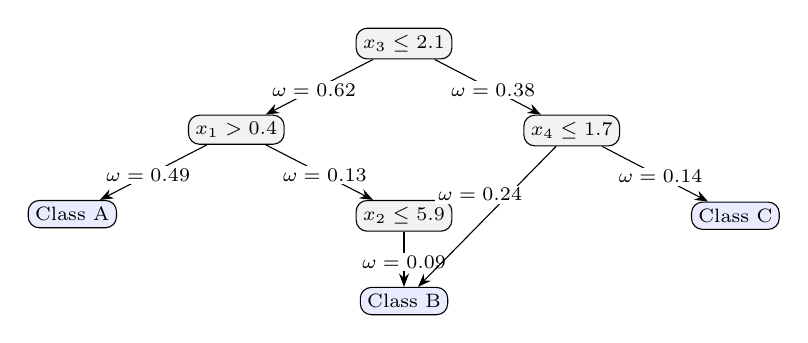
\begin{tikzpicture}[
  >=Stealth,
  node distance=7mm and 9mm,
  pred/.style={rectangle, rounded corners, draw=black, fill=gray!10, align=center, font=\scriptsize, inner sep=2.5pt},
  cls/.style={rectangle, rounded corners, draw=black, fill=blue!8, align=center, font=\scriptsize, inner sep=2.5pt},
  elab/.style={font=\scriptsize, fill=white, inner sep=1pt}
]
\node[pred] (p1) {$x_3 \le 2.1$};
\node[pred, below left=of p1] (p2) {$x_1 > 0.4$};
\node[pred, below right=of p1] (p3) {$x_4 \le 1.7$};
\node[pred, below right=of p2] (p4) {$x_2 \le 5.9$};
\node[cls, below left=of p2] (cA) {Class A};
\node[cls, below=of p4] (cB) {Class B};
\node[cls, below right=of p3] (cC) {Class C};
\draw[->] (p1) -- node[elab, pos=0.55] {$\omega=0.62$} (p2);
\draw[->] (p1) -- node[elab, pos=0.55] {$\omega=0.38$} (p3);
\draw[->] (p2) -- node[elab, pos=0.55] {$\omega=0.49$} (cA);
\draw[->] (p2) -- node[elab, pos=0.55] {$\omega=0.13$} (p4);
\draw[->] (p4) -- node[elab, pos=0.55] {$\omega=0.09$} (cB);
\draw[->] (p3) -- node[elab, pos=0.55, above, yshift=7pt] {$\omega=0.24$} (cB);
\draw[->] (p3) -- node[elab, pos=0.55] {$\omega=0.14$} (cC);
\end{tikzpicture}
\caption{Illustrative DPG-local graph for one sample. Rectangles are standardised predicate nodes, rounded blue rectangles are class terminals, and edge labels are normalised transition support.}
\label{fig:dpg-example}
\end{figure}




\subsection{Semantic Graph View} \label{sec:semantic-layer}
The DPG-local construction gives a trace-faithful local graph, but diagnosis requires compact quantities comparable across samples and datasets. We derive metrics targeting three needs: separation between predicted and competing classes, concentration of evidence, and agreement between the explanation and the ensemble decision. The confidence score aggregates these signals under structural coverage, so high confidence is reported only when both semantic support and trace recovery are strong.
From $G_x$, we extract weighted explanation paths $\mathcal{P}_x=\{(p,w_x(p),y(p))\}$, where $p$ is a local path, $w_x(p)\ge 0$ is its support, and $y(p)$ is its class endpoint. We normalize supports as $\tilde{w}_x(p)={w_x(p)}/{\sum_{q\in\mathcal{P}_x} w_x(q)+\varepsilon}$ with $\varepsilon=10^{-12}$. Class support $S_x(y)$ sums normalised path support over all paths ending in class $y$. The explanation class $\hat{y}^{exp}_x$ has largest support; the strongest competitor $y_x^{(2)}$ has highest remaining support.
The \emph{margin} $M_x=S_x(\hat{y}^{exp}_x)-S_x(y_x^{(2)})$ measures class separation. \emph{Path purity} $\mathrm{PathPurity}_x=S_x(\hat{y}^{exp}_x)$ and \emph{competitor exposure} $\mathrm{CompetitorExposure}_x=1-\mathrm{PathPurity}_x$ quantify support concentration.
\emph{Top-$K$ concentration} $C_x^{(K)}$ (with $K=3$) captures whether predicted-class evidence is dominated by a few paths. \emph{Vote agreement} $A_x=V_x(\hat{y}^{exp}_x)/B$ quantifies alignment with the ensemble vote, where $V_x(y)$ is the number of base learners voting for class $y$. \emph{Structural coverage} $G_x^{cov}=(R_x^{node}+R_x^{edge})/2$ summarizes trace recovery.
These are combined into the \emph{explanation confidence}:
\[
\mathrm{Conf}_x=G_x^{cov}\cdot\frac{M_x+C_x^{(K)}+A_x}{3}.
\]
The combination is scale-consistent: all four components lie in $[0,1]$, so $\mathrm{Conf}_x\in[0,1]$.
An unweighted mean of $(M_x,C_x^{(K)},A_x)$ avoids dataset-specific tuning.


\begin{table}[h!]
\centering
\small
\caption{Semantic Graph View metrics and their explainability use.}
\label{tab:semantic-metrics}
\setlength{\tabcolsep}{5pt}
\begin{tabular}{p{2.8cm} p{8.0cm}}
\toprule
Metric & Explainability use \\
\midrule
Class support & Quantifies evidence assigned to each class from local paths. \\
\addlinespace[1pt]
Pred./competitor class & Identifies the explained outcome and the strongest alternative for contrastive analysis. \\
\addlinespace[1pt]
Margin & Measures separation of predicted and competitor classes. \\
\addlinespace[1pt]
Path purity & Indicates how much support remains on the predicted class. \\
\addlinespace[1pt]
Comp. exposure & Indicates how much support shifts toward alternative classes. \\
\addlinespace[1pt]
Top-$K$ conc. & Shows evidence concentration of a few dominant paths. \\
\addlinespace[1pt]
Vote agreement & Checks alignment between the explanation class and the ensemble voting behaviour. \\
\addlinespace[1pt]
Structural coverage & Summarises node/edge recovery of executed traces. \\
\addlinespace[1pt]
Explanation conf. & Provides a compact summary of local explanation quality. \\
\bottomrule
\end{tabular}
\end{table}

Its coverage acts as a multiplicative reliability gate that down-weights strong semantic signals when trace recovery is weak.
This is not a probability-calibration measure but a compact summary of structural coverage, class separation, evidence concentration, and ensemble agreement. Table~\ref{tab:semantic-metrics} summarises all Semantic Graph View metrics and their explainability use.






\subsection{Critical Node and Structural Faithfulness}
\label{sec:structural-faithfulness}

We use the strongest predicted-class path $p_x^\ast$ and the strongest competitor path $q_x^\ast$ to localise where the explanation route diverges. Comparing the two ordered node sequences through their longest common prefix, the last shared non-root predicate is the \emph{critical node} $c_x$ at depth $d_x$ when such a shared predicate exists. Branch contrast $\Delta_x^{crit}=|B_x(s_x^{pred})-B_x(s_x^{comp})|$ measures post-split support divergence, where $B_x(\cdot)$ is normalized branch support after the critical split (Figure~\ref{fig:critical-node-example}). Under the current execution-trace construction this shared-prefix condition is rare, so critical nodes are treated as conditional contrastive descriptors rather than as a guaranteed component of every local explanation.

\textit{Structural faithfulness} is evaluated specifically against executed traces. Let $(T_x^{node},T_x^{edge})$ be trace node/edge sets and $(E_x^{node},E_x^{edge})$ the explanation sets. Node and edge recall/precision are intersection-over-trace-size and intersection-over-explanation-size, respectively ($\varepsilon=10^{-12}$ smoothing in denominators), complemented by the recombination rate defined in Section~\ref{sec:dpg-construction}.

\begin{figure}[h]
\centering
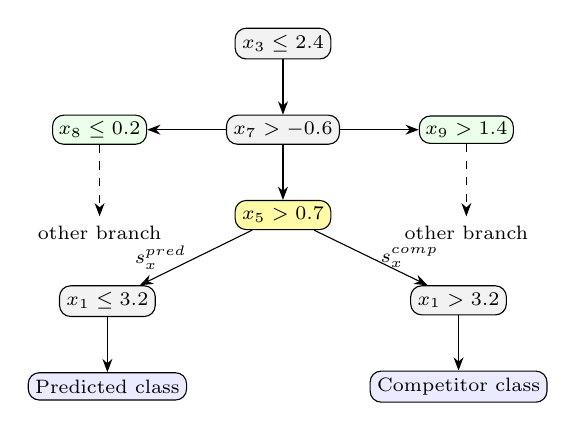
\begin{tikzpicture}[
  >=Stealth,
  node distance=7.0mm and 10.0mm,
  pred/.style={rectangle, rounded corners, draw=black, fill=gray!10, align=center, font=\scriptsize, inner sep=2.5pt},
  crit/.style={rectangle, rounded corners, draw=black, fill=yellow!35, align=center, font=\scriptsize, inner sep=2.5pt},
  cls/.style={rectangle, rounded corners, draw=black, fill=blue!8, align=center, font=\scriptsize, inner sep=2.5pt},
  side/.style={rectangle, rounded corners, draw=black, fill=green!8, align=center, font=\scriptsize, inner sep=2.2pt}
]
\node[pred] (p1) {$x_3 \le 2.4$};
\node[pred, below=of p1] (p2) {$x_7 > -0.6$};
\node[crit, below=of p2] (c) {$x_5 > 0.7$};
\node[pred, below left=of c] (pp1) {$x_1 \le 3.2$};
\node[cls, below=of pp1] (yp) {Predicted class};
\node[pred, below right=of c] (pc1) {$x_1 > 3.2$};
\node[cls, below=of pc1] (yc) {Competitor class};
\node[side, left=of p2] (s1) {$x_8 \le 0.2$};
\node[side, right=of p2] (s2) {$x_9 > 1.4$};
\draw[->] (p1) -- (p2);
\draw[->] (p2) -- (c);
\draw[->] (p2) -- (s1);
\draw[->] (p2) -- (s2);
\draw[->] (c) -- node[font=\scriptsize, left] {$s_x^{pred}$} (pp1);
\draw[->] (c) -- node[font=\scriptsize, right] {$s_x^{comp}$} (pc1);
\draw[->] (pp1) -- (yp);
\draw[->] (pc1) -- (yc);
\draw[dashed,->] (s1) -- ++(0,-1.1) node[below,font=\scriptsize] {other branch};
\draw[dashed,->] (s2) -- ++(0,-1.1) node[below,font=\scriptsize] {other branch};
\end{tikzpicture}
\caption{Illustration of Critical-node: two strongest paths share prefix $x_3 \le 2.4 \to x_7 > -0.6 \to$ critical node, but diverge in predicted and competitor successors. Side branches show that alternative paths, not part of the two strongest,  coexist in the local graph.}
\label{fig:critical-node-example}
\end{figure}

% -----------------------------------------------------------------------
\section{Experimental Setup}
% -----------------------------------------------------------------------

\subsection{Datasets and Models}
We evaluate our method on 15 numeric tabular  datasets for classification tasks: \texttt{banknote-authentication}, \texttt{breast\_cancer}, \texttt{diabetes}, \texttt{digits}, \texttt{ionosphere}, \texttt{iris}, \texttt{isolet}, \texttt{madelon}, \texttt{phoneme}, \texttt{qsar-biodeg}, \texttt{segment}, \texttt{spambase}, \texttt{vehicle}, \texttt{wdbc}, and \texttt{wine} (Table~\ref{tab:datasets-models-summary}). These cover binary and multiclass tasks with very different feature counts and levels of predicate reuse, important for evaluating structural faithfulness on both simple and harder ensemble decision boundaries. The final-test evaluation uses the complete locked test split for every dataset, corresponding to $6{,}079$ test samples per method; no per-dataset subsampling is applied in the main final-test comparison.
For every dataset we train random forest classifiers with search space $n_{\mathrm{estimators}} \in \{10,20\}$, $\mathrm{max\_depth}=4$, $\mathrm{perc\_var} \in \{10^{-4},10^{-5}\}$, and $\mathrm{decimal\_threshold}=6$, where $\mathrm{perc\_var}$ is the minimum path-frequency ratio used to keep predicate transitions in the DPG construction pipeline, and $\mathrm{decimal\_threshold}$ is the number of decimal digits used to round split thresholds when predicates are standardized. Each configuration is repeated with seeds $27$ and $42$. The best DPG-local configuration per dataset is selected by ranking runs on local match rate ($\mathrm{local\_matches\_model\_rate}$, the fraction of samples where the explanation class equals the model-predicted class), edge precision, node precision, recombination rate, and explanation confidence, in that order.

To assess whether the diagnostic representation is restricted to random forests, we also evaluate execution-trace DPGs across four DPG-compatible classification ensemble families: RandomForest, ExtraTrees, AdaBoost with tree base learners, and Bagging with tree base learners. This model-family experiment uses the same 15 datasets, the final test split, 20 estimators, depth 4, and 10 random seeds ($27,42,100,101,102,103,104,105,106,107$), yielding 600 completed runs. The model-family study is therefore limited to a coherent set of vote-based tree classification ensembles. Additive gradient-boosted families are excluded intentionally, because their path aggregation semantics differ from class-vote ensembles and require a separate adapter.


\begin{table}[t]
  \centering
  \small
  \caption{Dataset and model summary. `Test' is the number of locked final-test samples used per method. `Avg.\ RF Perf.' is averaged across configurations and seeds.}
  \label{tab:datasets-models-summary}
  \begin{tabular}{lccccc}
    \toprule
    Dataset & \#Classes & \#Features & \#Samples & Test & Avg. RF Perf. \\
    \midrule
    banknote-authentication & 2 & 4 & 1372 & 275 & 0.963 \\
    breast\_cancer & 2 & 30 & 569 & 114 & 0.950 \\
    diabetes & 2 & 8 & 768 & 154 & 0.726 \\
    digits & 10 & 64 & 1797 & 360 & 0.848 \\
    ionosphere & 2 & 34 & 351 & 71 & 0.939 \\
    iris & 3 & 4 & 150 & 30 & 0.944 \\
    isolet & 26 & 617 & 7797 & 1560 & 0.714 \\
    madelon & 2 & 500 & 2600 & 520 & 0.626 \\
    phoneme & 2 & 5 & 5404 & 1081 & 0.818 \\
    qsar-biodeg & 2 & 41 & 1055 & 211 & 0.816 \\
    segment & 7 & 19 & 2310 & 462 & 0.850 \\
    spambase & 2 & 57 & 4601 & 921 & 0.906 \\
    vehicle & 4 & 18 & 846 & 170 & 0.695 \\
    wdbc & 2 & 30 & 569 & 114 & 0.956 \\
    wine & 3 & 13 & 178 & 36 & 0.987 \\
    \bottomrule
  \end{tabular}
\end{table}


\subsection{Compared Methods, Metrics, and Statistical Analysis}
The main comparison includes DPG-local, DPG-global, and five route-, rule-, or surrogate-relevant baselines: TreeSHAP, LIME, Anchors, a LORE-style local surrogate, and a tree-path baseline aggregating class-probability changes along executed tree paths. This mix covers model-direct, local-surrogate, and rule-based families. TreeSHAP, tree-path, and Anchors are evaluated on the trained random forest directly; LIME and the LORE-style baseline provide local-surrogate reference points. The LORE-style baseline samples a local neighbourhood around the query point, labels it with the trained forest, fits a shallow local decision-tree surrogate, and reports both the local rule and a nearest opposite-label counterfactual summary. ICE is reported separately in Appendix~\ref{app:ice}, because it is a response-profile diagnostic and does not return a local route, rule, path, or transition object.
Baseline hyperparameters: TreeSHAP uses 200 background instances; LIME uses 20 explanation features and 1000 perturbed samples; Anchors uses precision target $0.95$, maximum rule length 4, and at most 12 candidate conditions per expansion step. The LORE-style surrogate uses the same trained forest as oracle for the synthetic neighbourhood. The appendix ICE diagnostic uses 21 grid points.
Appendix~\ref{app:scoring-interface} documents how each explainer's native output is mapped into the common scoring interface used by the shared metrics.
We report \emph{fidelity} (fraction where the explained class matches the model prediction), \emph{local accuracy} (fraction where the explained class matches the ground-truth label), and \emph{margin} (difference between the top explained-class score and the strongest competitor score) \cite{vilone2021notions,nauta2023anecdotal,doshi2017rigorous,miller2019explanation}. We also report \emph{sufficiency}, which keeps only the explanation-selected features, replaces the remaining features with a training-set reference, and measures the target-class probability, and \emph{comprehensiveness} \cite{nauta2023anecdotal}, which removes selected features and measures the probability drop. The semantic-faithfulness protocol allocates the same feature budget to all methods.

\subsubsection{DPG-local-Specific Metrics.}
Beyond shared metrics, only DPG-local is evaluated on node/edge recall\slash precision, recombination rate, explanation confidence, critical-node metrics (split depth, branch contrast), disagreement-aware cohort summaries, and critical-branch intervention metrics. The cohort analysis separates model-correct/explanation-correct (MC-EC), model-wrong/explanation-matches-model (MW-EM), and disagreement cases. Critical-node quantities are reported as bounded diagnostics because they require a non-root shared prefix between predicted and competitor paths; in the present journal study this condition is mainly observed in aggregated DPGs rather than in execution-trace graphs.

\subsubsection{Statistical Analysis}
Results are reported at the dataset level unless stated otherwise. Aggregation is performed after per-dataset best-configuration selection. Sample-level summaries are used only when the unit of interpretation is an explanation object, as in readability and nearest-neighbour stability. We use the Friedman test for global method differences and paired Wilcoxon signed-rank tests for DPG-local vs.\ each baseline. Confidence intervals are reported for the main aggregate summaries, and Holm correction is applied to paired tests. All experiments were executed on the same multi-core server under a fixed parallel-execution protocol.


% -----------------------------------------------------------------------
\section{Results}
% -----------------------------------------------------------------------
\begin{figure}[ht!]
  \centering
  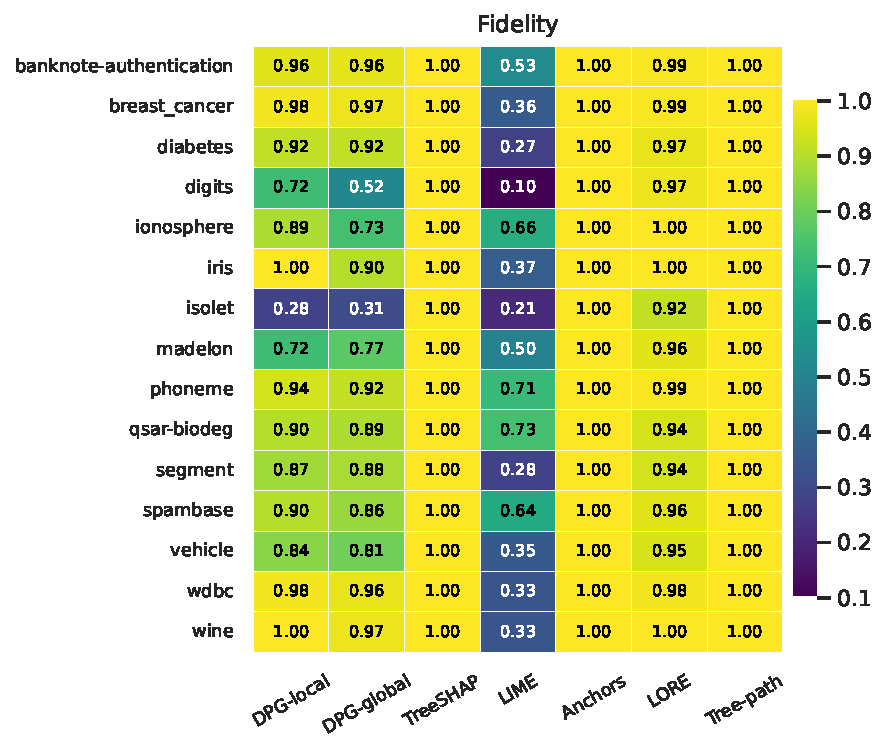
\includegraphics[width=\textwidth]{per_dataset_fidelity_heatmap.pdf}
  \caption{Per-dataset fidelity heatmap. Rows are datasets, columns are methods, including DPG-local, DPG-global, TreeSHAP, LIME, Anchors, LORE, and Tree-path; darker cells indicate higher values. ICE is excluded from this main route/path comparison and reported in Appendix~\ref{app:ice}.}
  \label{fig:per-dataset-fidelity}
\end{figure}

\begin{figure}[ht!]
  \centering
  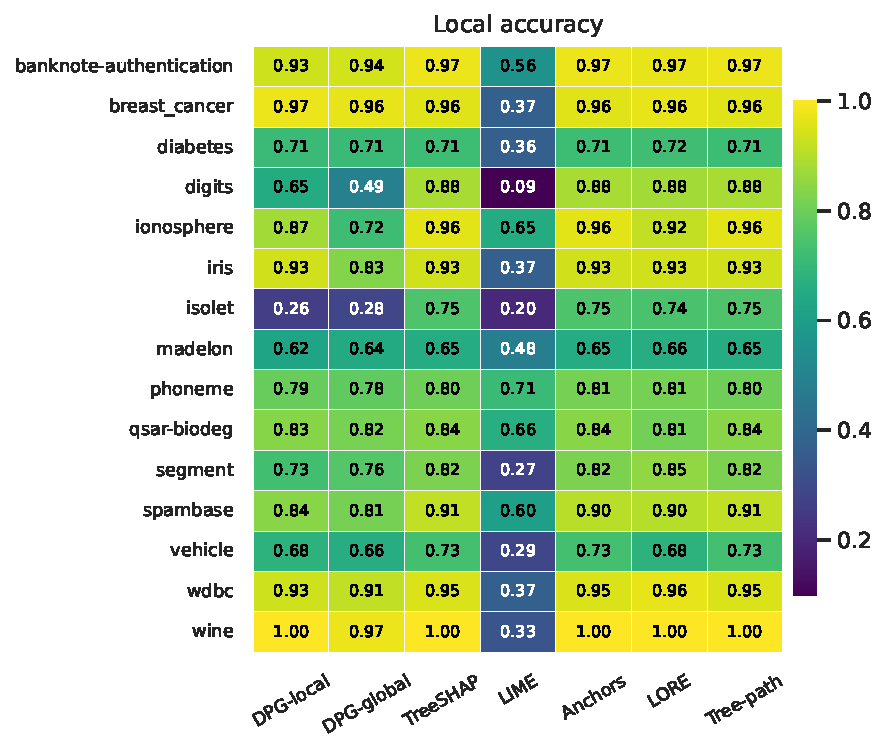
\includegraphics[width=\textwidth]{per_dataset_local_accuracy_heatmap.pdf}
  \caption{Per-dataset local-accuracy heatmap. Rows are datasets and columns are methods; darker cells indicate higher values.}
  \label{fig:per-dataset-local-accuracy}
\end{figure}

\begin{figure}[ht!]
  \centering
  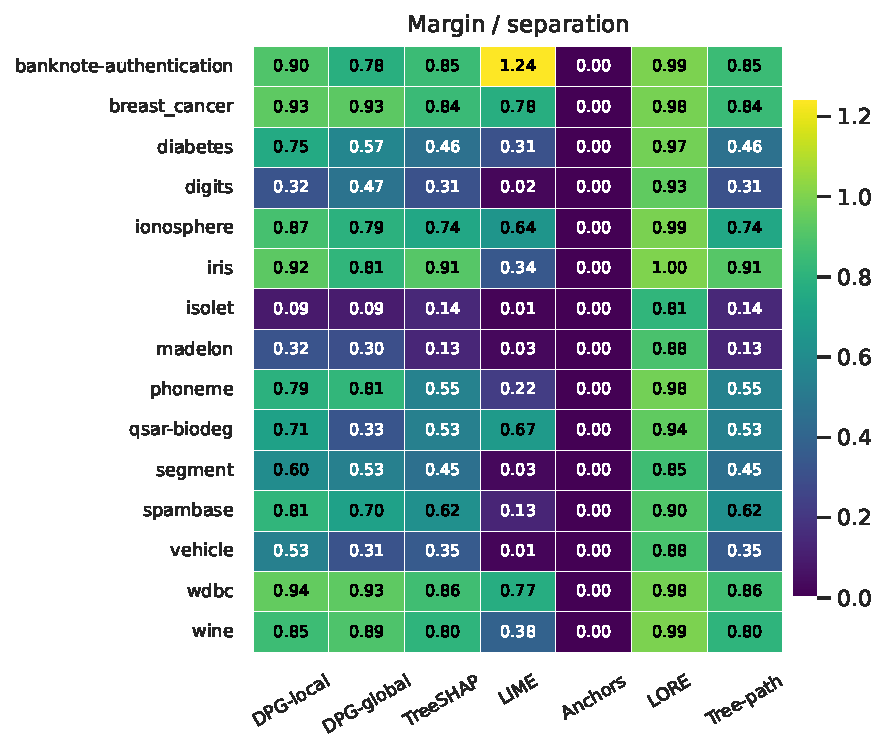
\includegraphics[width=\textwidth]{per_dataset_margin_heatmap.pdf}
  \caption{Per-dataset margin/separation heatmap. Rows are datasets and columns are methods; darker cells indicate higher values.}
  \label{fig:per-dataset-margin}
\end{figure}

\subsection{Baseline Comparison on Shared Metrics}
The results in Figures~\ref{fig:per-dataset-fidelity}--\ref{fig:per-dataset-margin} compare optimisation targets, not a single ranking. TreeSHAP, Tree-path, and Anchors dominate fidelity and local accuracy because they are explicitly designed to preserve model predictions. DPG-local is optimised for structural faithfulness (a surrogate representation), so lower fidelity relative to output-aligned baselines is expected. On margin, Anchors scores near zero because it returns a sufficient predicted-class rule without graded competitor decomposition, whereas DPG-local provides an explicit predicted-versus-competitor path-support decomposition.



The Friedman test rejects equal performance across datasets for the shared output-level metrics. Paired Wilcoxon tests confirm that DPG-local is below TreeSHAP and tree-path on fidelity ($p=0.0015$) and local accuracy ($p=0.0042$ for both comparisons). The same pattern holds for Anchors and path-control baselines, which are designed to preserve the model output. Conversely, DPG-local is substantially above LIME on fidelity and local accuracy ($p<10^{-3}$ after Holm correction). ICE is not included in this main route/path ranking and is discussed in Appendix~\ref{app:ice}.

The controlled internal ablation between the aggregated DPG and execution-trace DPG directly supports the main design claim. Across 15 datasets, execution-trace DPG improves mean fidelity from $0.825$ to $0.860$, mean local accuracy from $0.752$ to $0.783$, mean confidence from $0.477$ to $0.654$, and mean support margin from $0.617$ to $0.689$. It also reduces mean recombination from $0.134$ to zero. Dataset-level wins are 10/15 for fidelity, 10/15 for local accuracy, 11/15 for support margin, and 15/15 for confidence. DPG-local should therefore be interpreted as complementary to TreeSHAP and tree-path: it adds a structure-aware diagnostic view, including branch topology, competitor exposure, and critical-node descriptors, rather than targeting the same objective as output-fidelity explainers.

\subsection{Semantic Faithfulness}

This subsection focuses on DPG-local and LIME because they are directly
comparable under the same perturbation-based, matched feature-budget protocol. The focused semantic-faithfulness analysis contains 2,975 evaluated instances across the 15 datasets. Here, the comprehensiveness drop denotes the decrease in the predicted class
probability after removing the features selected by the explanation; higher
values indicate that the selected subset captures features on which the model
more strongly relies. Under this subgroup protocol, DPG-local reaches a mean
sufficiency probability of $0.54$ and a mean comprehensiveness drop of $0.13$,
close to LIME ($0.55$ and $0.17$) (Table~\ref{tab:semantic-faithfulness}). The corresponding ICE response-profile values are reported in Appendix~\ref{app:ice}.


\subsection{Structural Faithfulness, Disagreement, and Misclassification}

Structural metrics are the dimension in which DPG-local construction provides its main advantage. Since there is no directly comparable graph-based baseline in our setting, this subsection reports a DPG-local-centred structural evaluation across datasets. In the dataset-level final-test summary, execution-trace DPG explanations contain on average $20.00$ active paths and $63.96$ active nodes, while preserving the executed model structure almost exactly: mean edge precision is $1.00$, mean edge recall is $0.9999$, and mean recombination is $0.00$ (Table~\ref{tab:dpg-structural}). Under DPG-local construction, edge precision and recombination are expected consistency checks because only executed edges are inserted. The key empirical structural result is therefore near-complete edge recall, which confirms that the constructed local graph retains almost all executed transitions in practice.


\begin{table}[ht!]
  \centering
  \small
  \caption{Semantic-faithfulness comparison for the focused subgroup
    (DPG-local, LIME) under the matched feature-budget protocol. Higher
    sufficiency probability and comprehensiveness drop are better.}
  \label{tab:semantic-faithfulness}
  \begin{tabular}{lcc}
    \toprule
    Method                    & Sufficiency Prob. & Comprehensiveness Drop \\
    \midrule
    DPG-local & 0.54             & 0.13 \\
    LIME                      & 0.55             & 0.17 \\
    \bottomrule
  \end{tabular}
\end{table}

\begin{table}[ht!]
\centering
\small
\caption{DPG-local structural and semantic diagnostics. Edge precision/recombination are construction-consistency checks; edge recall and cohort/disagreement shifts are the main empirical diagnostics.}
\label{tab:dpg-structural}
\begin{tabular}{lcccccc}
\toprule
Group & Conf. & Margin & Purity & Comp. Exp. & Edge Prec. & Recomb. \\
\midrule
Overall  & 0.65 & 0.69 & 0.81 & 0.19 & 1.00 & 0.00 \\
Agree    & 0.66 & 0.69 & 0.81 & 0.19 & n/a  & 0.00 \\
Disagree & 0.40 & 0.11 & 0.38 & 0.62 & n/a  & 0.00 \\
MC-EC    & 0.68 & 0.73 & 0.84 & 0.16 & 1.00 & 0.00 \\
MW-EM    & 0.55 & 0.47 & 0.68 & 0.32 & 1.00 & 0.00 \\
\bottomrule
\end{tabular}
\end{table}

Mean explanation confidence is $0.654$ in the dataset-level final-test summary, ranging from $0.392$ (\texttt{isolet}) to $0.788$ (\texttt{banknote-authentication}), reflecting dataset difficulty. The dominant cohort is MC-EC, which accounts for $61.3\%$ of evaluated samples and has mean confidence $0.676$, path purity $0.839$, and competitor exposure $0.161$. Model-wrong explanations that still match the model prediction (MW-EM) remain moderately confident, with confidence $0.546$ and path purity $0.678$, showing that a structurally coherent explanation can still support the wrong class when the ensemble itself is wrong.
The disagreement split is the most informative result. Agreement cases show confidence $0.656$, margin $0.691$, and model-vote agreement $0.813$; disagreement cases drop to $0.399$, $0.112$, and $0.255$ respectively, despite near-perfect trace coverage in both groups. Competitor exposure rises from $0.186$ in agreement cases to $0.622$ in disagreement cases. Disagreement is thus not random noise but a measurable redistribution of support toward competing branches.
Critical-node evidence is much weaker than the disagreement evidence. Under the current non-root shared-prefix definition, the 15-dataset validation finds no eligible critical nodes in execution-trace DPGs, whereas aggregated DPGs show them in about $19.6\%$ of held-out samples with a pooled changed-to-competitor rate of $0.025$. We therefore keep critical nodes as a bounded structural descriptor of the broader DPG family rather than as a validated core diagnostic of execution-trace DPG-local.

\subsection{Confidence Sensitivity and Diagnostic Value}

The confidence score is intended as a diagnostic ranking index, not a calibrated probability. To test whether the conclusion depends on the exact unweighted formula in Section~\ref{sec:semantic-layer}, we evaluate alternative risk scores for local disagreement, including low reported confidence, low vote agreement, low margin, high competitor exposure, low path purity, and variants with different structural-coverage gates. The reported low-confidence score remains strong: for execution-trace DPGs, low confidence predicts local disagreement with AUROC $0.9046$ and AUPRC $0.6509$ across the 15 datasets. Low vote agreement is even stronger, with AUROC $0.9808$ and AUPRC $0.9104$, while competitor exposure and margin-only scores also retain useful signal. Concentration-only is not merely weak but anti-predictive in execution-trace mode, with AUROC $0.0876$, so it should be interpreted as an evidence-distribution descriptor rather than as a disagreement detector.

The same diagnostic family also carries information about model error. For execution-trace DPGs, low reported confidence predicts model misclassification with AUROC $0.7523$ and AUPRC $0.3216$ on a mean positive rate of about $0.144$, while vote agreement again performs best (AUROC $0.7638$, AUPRC $0.3417$). This is weaker than disagreement detection, but still useful as a ranking signal for cases where the ensemble is more likely to be wrong.

This sensitivity analysis changes the interpretation of confidence in a useful way. The contribution is not the particular arithmetic form of a single confidence score; rather, the DPG graph exposes a family of local diagnostic variables. Vote agreement, support margin, competitor exposure, path purity, and structural coverage jointly distinguish stable explanations from contested ones. The ranking itself is highly stable: for execution-trace DPGs, the reported low-confidence ranking has Spearman $\rho=1.0$ with multiplicative-gate, additive-coverage, and no-gate variants, $\rho=0.954$ with margin-only, and $\rho=0.919$ with vote-agreement-only. This justifies keeping the simple formula while avoiding an overclaim of probabilistic calibration. Empirically, the score separates low-risk from moderate-risk cases well, but the highest-risk bins are not perfectly monotonic, so we use it strictly as an ordinal diagnostic index.

\subsection{Local Stability Under Nearest-Neighbour Perturbations}

We further evaluate local robustness by comparing each final-test explanation with the explanations of its five nearest neighbours in standardized input space, computed within the same dataset and final test split. This analysis does not perturb features independently; instead, it asks whether naturally similar samples receive similar explanation labels and diagnostic values. Across 30,395 nearest-neighbour pairs for execution-trace DPGs, explained-label agreement is $0.785$, close to the corresponding model-label agreement of $0.795$. The median absolute changes in the main diagnostic quantities are small: $0.024$ for explanation confidence, $0.044$ for support margin, $0.029$ for competitor exposure, and $0.050$ for vote agreement.

The same experiment also shows that DPG diagnostics change gradually with input distance. For execution-trace DPGs, Spearman correlations between neighbour distance and absolute diagnostic change are $\rho=0.234$ for confidence, $\rho=0.291$ for support margin, $\rho=0.326$ for competitor exposure, and $\rho=0.249$ for vote agreement. These correlations are moderate rather than large, which is expected because nearest neighbours may still cross class boundaries in difficult datasets. The result nevertheless supports the use of DPG diagnostics as local stability indicators: nearby samples tend to preserve labels and diagnostic scores when the model decision is stable, while larger diagnostic shifts identify locally contested regions.

\subsection{Dataset and Model Regimes}

The regime analysis combines final-test diagnostics, confidence sensitivity, scalability, and the 10-seed model-family evaluation. Table~\ref{tab:regime-summary} summarises the main pattern. DPG diagnostics are strongest on low- to moderate-dimensional binary datasets and small multiclass datasets where support is concentrated and competitor exposure is low. They are weakest in many-class or high-dimensional regimes, where multiple class endpoints receive substantial support even when trace recovery remains high.

\begin{table}[ht!]
\centering
\scriptsize
\setlength{\tabcolsep}{3pt}
\caption{Dataset/model regimes for execution-trace DPG diagnostics. Local match is the rate at which the DPG explanation class matches the model prediction. Vote agr.\ is mean model-vote agreement and Comp.\ exposure is mean competitor exposure.}
\label{tab:regime-summary}
\resizebox{\textwidth}{!}{%
\begin{tabular}{l l c c c c}
\toprule
Regime & Example datasets & Local match & Conf. & Vote agr. & Comp.\ exposure \\
\midrule
Low-dim.\ binary & banknote, diabetes, phoneme & 0.94 & 0.72 & 0.88 & 0.09 \\
Low-dim.\ multiclass & iris & 1.00 & 0.73 & 0.93 & 0.04 \\
Moderate binary & breast cancer, wdbc, spambase & 0.93 & 0.73 & 0.92 & 0.07 \\
Moderate many-class & digits & 0.72 & 0.50 & 0.54 & 0.47 \\
High-dim.\ binary & madelon & 0.72 & 0.49 & 0.62 & 0.34 \\
High-dim.\ many-class & isolet & 0.28 & 0.39 & 0.32 & 0.69 \\
\bottomrule
\end{tabular}
}
\end{table}

This pattern prevents an overgeneral interpretation of the method. DPG-local is not uniformly strong in every setting. Instead, it provides an auditable diagnostic object whose variables reveal when the local decision is stable, contested, expensive, or weak. In \texttt{isolet}, for example, local match is only $0.2776$, confidence is $0.3921$, competitor exposure is $0.6860$, and the disagreement rate is $0.7224$. In \texttt{madelon}, the outcome is less severe but still boundary-like: local match is $0.7212$, confidence is $0.4931$, and competitor exposure is $0.3385$. These values do not merely indicate lower aggregate performance; they identify local decision regimes in which DPG diagnostics should be interpreted together with output-aligned explainers.

\subsection{Supported Model Families and Scalability}

The model-family experiment confirms that execution-trace DPGs are not limited to a single random-forest setting. Across 15 datasets, four ensemble families, and 10 seeds, all 600 runs completed without local failures. Edge recall remains close to one and recombination remains zero for every family (Table~\ref{tab:model-family}). This result supports the structural stability of the execution-trace construction across several vote-based tree-ensemble classifiers, but should not be extrapolated to additive gradient-boosted models without a separate adapter.

The diagnostic quantities, however, are not invariant across model families. Bagging gives the highest mean local match ($0.899$) and the lowest competitor exposure ($0.132$), followed by RandomForest ($0.865$, exposure $0.180$), ExtraTrees ($0.807$, exposure $0.244$), and AdaBoost ($0.725$, exposure $0.279$). The gap is not uniform noise. On \texttt{phoneme}, AdaBoost reaches local match $0.369$ whereas Bagging reaches $0.923$; on \texttt{spambase}, the same contrast is $0.675$ versus $0.981$; and on \texttt{isolet}, AdaBoost falls to $0.153$. Thus, trace recovery is stable, while the concentration of local support depends strongly on both the ensemble family and the dataset. This distinction is important: the graph construction can be structurally reliable even when the local decision remains contested.

\begin{table}[ht!]
\centering
\small
\caption{Execution-trace DPG results across model families. Values are means over 15 datasets and 10 seeds per family.}
\label{tab:model-family}
\begin{tabular}{lcccccc}
\toprule
Family & Local match & Local acc. & Conf. & Comp.\ exp. & Edge recall & Recomb. \\
\midrule
AdaBoost      & 0.725 & 0.692 & 0.634 & 0.279 & 0.999 & 0.000 \\
Bagging       & 0.899 & 0.799 & 0.675 & 0.132 & 0.999 & 0.000 \\
ExtraTrees    & 0.807 & 0.703 & 0.592 & 0.244 & 0.999 & 0.000 \\
RandomForest  & 0.865 & 0.786 & 0.661 & 0.180 & 0.999 & 0.000 \\
\bottomrule
\end{tabular}
\end{table}

We also compare the size of the explanation objects produced by DPG-local and path-based controls at the sample level. The execution-trace DPG contains on average 72.5 active nodes per explanation, whereas raw path-control representations require about 666 unique predicates on average and more than 1100 predicates at the 90th percentile (Table~\ref{tab:readability-cost}). Tree-path summaries are smaller, but they collapse the explanation to feature-level evidence and do not retain predicate-transition topology or predicted-versus-competitor branches. DPG-local therefore occupies an intermediate position: it is less compact than a feature ranking, but substantially more structured and more compact than a raw union of executed path predicates.

\begin{table}[ht!]
\centering
\small
\caption{Readability and size comparison. Display size is measured as active graph nodes for DPG-local, unique predicates for path controls, and selected features or rule length for non-graph methods when available. ``not meas.'' means that comparable per-sample runtime was not measured in this summary.}
\label{tab:readability-cost}
\begin{tabular}{lccc}
\toprule
Method & Mean display size & 90th percentile & Mean runtime (ms) \\
\midrule
Tree-path             & 3.9   & 4    & 3.8 \\
LORE-style surrogate  & 3.2   & 4    & 75.8 \\
TreeSHAP              & 55.0  & 127  & 8.2 \\
DPG-local             & 72.5  & 88   & not meas. \\
Path controls         & 666.4 & 1194 & 65.9 \\
\bottomrule
\end{tabular}
\end{table}

Scalability experiments further show the practical boundary of the method. At depth 4, execution-trace DPGs remain lightweight; under depth and ensemble-size stress, runtime and graph size grow sharply. For the depth-focused stress report, mean runtime rises from about $119$ ms at depth 4 to about $4.38$ s at depth 8 and $14.63$ s at depth 12; the hardest depth-12, 50-estimator cases reach tens of seconds on high-dimensional datasets such as \texttt{isolet}. Thus, DPG construction is trace-faithful but should be paired with pruning, sampling, or depth-aware deployment rules for large ensembles.

% -----------------------------------------------------------------------
\section{Discussion}
\label{sec:discussion}
% -----------------------------------------------------------------------

The results show that output-level agreement is an incomplete proxy for explanation quality when the goal is diagnosis rather than justification. Methods such as TreeSHAP, Anchors, and the tree-path baseline are designed to preserve the model output and therefore score strongly on fidelity and local accuracy, whereas DPG-local is designed to preserve the \emph{executed decision structure} and to expose class competition through an explicit local graph. This difference in optimisation targets clarifies how DPG-local should be interpreted in practice: it is not intended to replace attribution-based explanations, but to complement them when analysts need to inspect how a tree ensemble committed to a decision and where plausible alternatives were present. In such workflows, the explanation object matters because a graph of executed predicate transitions can be checked against the model trace and supports questions that are difficult to answer from feature contributions alone, including whether local support is concentrated or contested, where predicted and competitor routes diverge, and if disagreement coincides with a measurable redistribution of support toward alternative classes.

\emph{Structural findings.} The cohort analysis supports this interpretation: disagreement cases are associated with reduced confidence and margin and increased competitor exposure, while trace coverage remains essentially stable, indicating that disagreement reflects a redistribution of local support rather than a failure to recover the executed structure. Because DPG-local edges are formed only from executed traces, edge precision and recombination primarily act as construction-consistency checks, while edge recall and coverage capture whether the extracted local graph retains executed transitions in practice. The confidence sensitivity and nearest-neighbour stability results further show that the diagnostic signal is not tied to a single formula or to isolated samples: vote agreement, support margin, competitor exposure, and confidence all carry information about local disagreement, and the sample ranking is essentially unchanged under several alternative gate choices. Evaluation should therefore combine shared output-level metrics with structure-dependent criteria and semantic diagnostics rather than relying on a single fidelity score \cite{nauta2023anecdotal,doshi2017rigorous}.

\emph{Regime-dependent utility.} The dataset/model-regime analysis suggests that DPG-local is most useful when the local ensemble evidence is concentrated enough for a compact graph to expose a stable route, but still rich enough to reveal competitor branches. Low- and moderate-dimensional binary datasets and small multiclass datasets fit this profile. Many-class and high-dimensional datasets, especially \texttt{isolet}, are harder: the graph remains trace-faithful, but local evidence is diffuse and competitor exposure is high. This is a useful failure mode rather than a reason to discard the representation, because the diagnostics explicitly tell the analyst that the local decision is contested.

\emph{Critical nodes and contrastive reasoning.} Critical decision nodes are informative only when the strongest predicted and strongest competitor paths share a non-root prefix, and under the current execution-trace construction this condition is often absent. In the present results, critical nodes should therefore be treated as conditional boundary descriptors of the broader DPG family, not as causal explanations or as a primary contribution of DPG-local. Probability shifts toward the competitor class may provide a more sensitive signal of diagnostic relevance, but require a separate validation protocol.

\emph{Limitations.} On difficult datasets such as \texttt{isolet}, \texttt{digits}, and \texttt{madelon}, lower shared fidelity and higher competitor exposure indicate that DPG-local should be used together with output-aligned explainers when prediction-level agreement is the primary requirement. Scalability is another boundary: although per-sample complexity is linear in executed path length, very deep trees or very large ensembles can substantially increase local graph size and extraction latency, motivating support-threshold pruning strategies for deployment settings. Generalisation beyond the tested classification ensembles also requires methodological extensions: the current vote-agreement term is defined for class-vote ensembles, so additive gradient-boosted trees, probability-averaging ensembles, and regression tasks need alternative aggregation semantics and, for regression, a revised notion of competitor structure.

\emph{Future directions.} These limitations suggest several lines of future work. User-oriented validation is needed to quantify whether competitor exposure and conditional critical-node descriptors improve real debugging and auditing decisions beyond what is achievable with feature attribution or rule summaries alone. The confidence family warrants calibration research, since the current score is best interpreted as a ranking index even though its component diagnostics are robust. Sufficiency and comprehensiveness evaluations would benefit from conditional perturbation operators that reduce off-manifold effects on correlated features. Finally, extending DPG-local beyond the tested classification setting through surrogate models with explicit fidelity controls would broaden its applicability to other predictive tasks where path-level tracing remains tractable.


% -----------------------------------------------------------------------
\section{Conclusion}
% -----------------------------------------------------------------------

We proposed DPG-local, an execution-trace formulation of Decision Predicate Graphs for local diagnostic analysis in tree ensembles, together with a Semantic Graph View providing explanation confidence, support margin, competitor exposure, vote agreement, and conditional critical-node descriptors. The key design principle is that each local graph is built exclusively from the root-to-leaf paths executed by the ensemble for the inspected sample, avoiding the recombination artefacts that arise when transitions are aggregated globally.
Across 15 tabular datasets, DPG-local achieves near-complete transition recovery (edge recall $\approx0.99$) with zero recombination, while edge precision and recombination serve as construction-consistency checks. It does not dominate output-aligned methods on raw fidelity, but the internal DPG ablation shows consistent improvements in confidence, support margin, and recombination control. The disagreement, confidence-sensitivity, nearest-neighbour stability, model-family, readability, and regime analyses further demonstrate that DPG-derived quantities characterise prediction/explanation mismatch, identify contested local decisions, and expose when graph-based local diagnostics are likely to be useful or limited. These findings position DPG-local as a diagnostic layer for practitioners who need to inspect, audit, or contest tree-ensemble inferences at the path level.

\appendix
\section{Reproducibility Summary}
\label{app:reproducibility}

Table~\ref{tab:reproducibility-protocol} summarises the experimental protocol used for the journal results. The main final-test comparison uses the locked test split for all 15 datasets, with 6,079 evaluated test instances per method. Results are aggregated at the dataset level unless the analysis explicitly concerns explanation objects, as in readability and nearest-neighbour stability.

\begin{table}[h!]
\centering
\scriptsize
\caption{Reproducibility summary for the journal experiments.}
\label{tab:reproducibility-protocol}
\resizebox{\textwidth}{!}{%
\begin{tabular}{p{3.0cm} p{10.0cm}}
\toprule
Item & Specification \\
\midrule
Datasets & 15 numeric tabular classification datasets listed in Table~\ref{tab:datasets-models-summary}. \\
Main split & Locked final-test split; 6,079 test instances per method, with no per-dataset subsampling in the main final-test comparison. \\
Main random-forest grid & $n_{\mathrm{estimators}}\in\{10,20\}$, $\mathrm{max\_depth}=4$, $\mathrm{perc\_var}\in\{10^{-4},10^{-5}\}$, $\mathrm{decimal\_threshold}=6$, seeds 27 and 42. \\
Selected configuration rule & Per-dataset ranking by local match, edge precision, node precision, recombination rate, and explanation confidence. \\
Main baselines & TreeSHAP, LIME, Anchors, LORE-style local surrogate, tree-path, raw path union, path bag, and random same-size path control. ICE is appendix-only. \\
Model-family experiment & RandomForest, ExtraTrees, AdaBoost with tree base learners, and Bagging with tree base learners; 15 datasets, 10 seeds, 20 estimators, depth 4, 600 completed runs. \\
Semantic faithfulness & Focused matched feature-budget perturbation protocol with 2,975 evaluated instances across 15 datasets. \\
Stability analysis & Five nearest neighbours in standardized input space within each dataset final-test split; 30,395 nearest-neighbour pairs. \\
Statistical tests & Friedman tests for global differences and paired Wilcoxon signed-rank tests with Holm correction for paired comparisons. \\
\bottomrule
\end{tabular}
}
\end{table}

Table~\ref{tab:artifact-provenance} gives the journal-root artifacts from which the main numerical claims were audited. The semantic-faithfulness files are mirrored under the same journal result root and include a provenance README with SHA-256 checksums.

\begin{table}[h!]
\centering
\scriptsize
\caption{Journal-result artifact provenance. Paths are relative to the project root.}
\label{tab:artifact-provenance}
\resizebox{\textwidth}{!}{%
\begin{tabular}{p{3.2cm} p{9.8cm}}
\toprule
Analysis & Artifact path \\
\midrule
Final-test comparison & \url{experiments_local_explanation/results_journal_v1/journal_report_final_with_path_controls_and_critical/summary.md} \\
Selected final-test rows & \url{experiments_local_explanation/results_journal_v1/final_test_main_with_lore_path_controls/} \\
Confidence sensitivity & \url{experiments_local_explanation/results_journal_v1/confidence_sensitivity/summary.md} \\
Nearest-neighbour stability & \url{experiments_local_explanation/results_journal_v1/local_stability_knn/summary.md} \\
Readability and cost & \url{experiments_local_explanation/results_journal_v1/readability_cost_analysis/summary.md} \\
Model-family experiment & \url{experiments_local_explanation/results_journal_v1/model_family_all15_10seeds_test_report/summary.md} \\
Scalability stress test & \url{experiments_local_explanation/results_journal_v1/dpg_scalability_depth_focused_report/summary.md} \\
Critical-node validation & \url{experiments_local_explanation/results_journal_v1/critical_node_validation_final_fixed/summary.md} \\
Semantic faithfulness & \url{experiments_local_explanation/results_journal_v1/semantic_faithfulness/} \\
Numerical audit & \url{JOURNAL_paper/NUMERICAL_CONSISTENCY_AUDIT_2026-06-19.md} \\
\bottomrule
\end{tabular}
}
\end{table}

\section{Common Scoring Interface}
\label{app:scoring-interface}

Table~\ref{tab:common-scoring-interface} documents how the shared metrics are derived from each method's native output. This appendix is included because the compared explainers produce fundamentally different objects, and the benchmark is only auditable if the mapping from those objects to explained class, score, and size proxy is explicit.

\begin{table}[h!]
\centering
\scriptsize
\caption{Common scoring interface used for the shared metrics.}
\label{tab:common-scoring-interface}
\resizebox{\textwidth}{!}{%
\begin{tabular}{lllll}
\toprule
Method & Native object & Explained class & Score field(s) & Size proxy \\
\midrule
DPG-local & local graph from executed forest paths & graph-supported predicted class & confidence, support margin, competitor exposure & active graph nodes \\
TreeSHAP & per-class attribution vector & model-predicted class & predicted-vs-competitor score margin & non-zero attribution count \\
LIME & local linear surrogate coefficients & model-predicted class & predicted-vs-competitor score margin & non-zero coefficient count \\
Anchors & local precision rule & model-predicted class & anchor precision and coverage & rule length \\
LORE-style surrogate & local decision-tree rule and nearest counterfactual & model-predicted class & neighbourhood fidelity, counterfactual distance & rule length \\
Tree-path & executed-path feature ranking & model-predicted class & predicted-vs-competitor score margin & non-zero path-feature count \\
Path controls & raw or bagged executed predicates & model-predicted class & predicted-vs-competitor score margin & predicate count \\
ICE & one-feature response profile & model-predicted class & probability range and slope & one varied feature \\
\bottomrule
\end{tabular}
}
\end{table}

\section{ICE as a Response-Profile Diagnostic}
\label{app:ice}

Individual Conditional Expectation (ICE) is useful for inspecting one-feature response profiles, but it is not a local route, rule, path, or graph explainer. It varies one feature over a grid while holding the remaining feature values fixed, and therefore answers a different question from DPG-local: how the model response changes along a selected coordinate, rather than which predicate transitions were executed by the ensemble for the inspected sample. For this reason, we do not use ICE as a main comparator in the route/path explanation ranking.

We nevertheless retain ICE as an ancillary diagnostic to document response-profile behaviour under the same experimental setting. ICE uses 21 grid points. Under the matched feature-budget semantic-faithfulness protocol, ICE obtains a mean sufficiency probability of $0.48$ and a mean comprehensiveness drop of $0.07$. These values are reported for completeness, but they should be interpreted as response-profile diagnostics rather than as evidence for or against structural path faithfulness.

\begin{table}[h!]
\centering
\small
\caption{Appendix ICE diagnostic. ICE is reported as a response-profile method, not as a route/path explainer.}
\label{tab:ice-appendix}
\begin{tabular}{lccc}
\toprule
Method & Diagnostic object & Sufficiency Prob. & Comprehensiveness Drop \\
\midrule
ICE & one-feature response profile & 0.48 & 0.07 \\
\bottomrule
\end{tabular}
\end{table}

\bibliographystyle{plain}
\bibliography{bibliography}

\end{document}
